\section{Características del equipo}
A fin de definir el alcance del desarrollo y permitir la verificación objetiva del desempeño del instrumento, se establecen a continuación las especificaciones técnicas del equipo. Estas especificaciones constituyen los requisitos mínimos a cumplir y permiten comparar el resultado obtenido con instrumentos equivalentes del segmento de laboratorio y enseñanza.

\subsection{Configuración general}

\begin{itemize}
	\item \textbf{Cantidad de canales:} 2 canales de salida independientes y sincronizables.
\end{itemize}

\subsection{Especificaciones de alimentación}

La fuente de alimentación deberá permitir el correcto funcionamiento del sistema en las condiciones nominales de operación, incluyendo la provisión de rieles de tensión para las etapas digitales y analógicas.

\begin{itemize}
	\item \textbf{Rango de tensión de entrada:} $V_{ac}$ = 85 a 265 Vrms (alimentación universal).
	\item \textbf{Potencia máxima de entrada:} $P_{in,max}$ = 70 W.
\end{itemize}

\subsection{Especificaciones de forma de onda}

Se definen a continuación las especificaciones eléctricas mínimas de salida del instrumento:

\begin{itemize}
	\item \textbf{Tensión pico a pico máxima:} $V_{pp,max} =$ 20 Vpp en High-Z y 10 Vpp en 50 $\Omega$.
	\item \textbf{Tensión de pico máxima:} $V_{p,max} =$ 15 V en High-Z y 7.5 V en 50 $\Omega$.
	\item \textbf{Resolución de amplitud:} $\leq 100$ mVp.
	\item \textbf{Corriente máxima de salida:} $I_{o,max} \geq 100$ mA.
	\item \textbf{Impedancia de salida:} $Z_o = 50\,\Omega$.
	\item \textbf{Frecuencia máxima de salida:} $f_{max} \simeq$ 15 MHz (senoidal), 10 MHz (cuadrada/triangular) y 10 MHz (arbitraria).
	\item \textbf{Resolución de frecuencia:} $\leq 1$ Hz.
	\item \textbf{Generación arbitraria:} la forma arbitraria deberá permitir al menos $N \ge 16$ muestras por período a la frecuencia máxima especificada.
\end{itemize}

\subsection{Formas de onda disponibles}
El instrumento deberá permitir la generación de las siguientes formas de onda en cada canal de salida:

\begin{itemize}
	\item \textbf{Senoidal}
	\item \textbf{Cuadrada}, con ciclo de trabajo ajustable
	\item \textbf{Triangular}
	\item \textbf{Diente de sierra}, ascendente y descendente
	\item \textbf{Forma arbitraria} definida por el usuario
	\item \textbf{Señal continua (DC)}
\end{itemize}

Cada forma de onda deberá ser configurable en términos de frecuencia, amplitud y offset dentro de los rangos especificados en las subsecciones correspondientes.

\subsection{Interfaz de usuario}

\begin{itemize}
	\item \textbf{Pantalla gráfica:} display gráfico integrado para visualización de parámetros y forma de onda.
	\item \textbf{Método de control:} encoder rotativo incremental y pulsadores dedicados.
\end{itemize}

\subsection{Conectividad}

El instrumento deberá incorporar interfaces de comunicación destinadas a su integración con sistemas externos.

\begin{itemize}
	\item \textbf{Interfaz USB:}
	\begin{itemize}[label=\textbullet]
		\item Compatible con estándar USB 1.1 o superior.
		\item Comunicación serial virtual (CDC o equivalente).
		\item Soporte para actualización de firmware.
	\end{itemize}
	
	\item \textbf{Interfaz Ethernet:}
	\begin{itemize}[label=\textbullet]
		\item Compatibilidad con estándar 10/100 Mbps.
		\item Soporte para comunicación TCP/IP.
	\end{itemize}
\end{itemize}

\section{Arquitectura de implementación}
Con el fin de cumplir con las especificaciones definidas en la Sección 3, se propone una arquitectura modular dividida en dos grandes bloques: \textbf{Hardware} y \textbf{Firmware}.

\subsection{Arquitectura de Hardware}
El sistema se organiza en tres placas principales:

\begin{itemize}
	\item \textbf{Placa de Control}
	\item \textbf{Placa de Alimentación}
	\item \textbf{Placa de Panel Frontal}
\end{itemize}

\paragraph{Placa de Control:} integra los siguientes bloques funcionales (Figura \ref{fig:awgdds}):

\begin{itemize}[label=\textbullet]
	\item Núcleo de síntesis DDS.
	\item Unidad de control digital (microcontrolador).
	\item Etapa de conversión corriente–tensión diferencial.
	\item Conversión diferencial a simple.
	\item Control de amplitud (ajuste grueso y fino).
	\item Etapa de offset DC.
	\item Amplificación final y adaptación a 50 $\Omega$.
	\item Generación de reloj.
	\item Memoria no volátil.
	\item Etapa de alimentación y filtrado.
	\item Comunicación USB y/o LAN Ethernet.
	\item Comunicación con panel frontal.
\end{itemize}

\paragraph{Placa de alimentación:} provee los rieles simétricos y digitales necesarios para el correcto funcionamiento de las etapas analógicas y de control (Figura \ref{fig:panelalimentaciondds}).

\paragraph{Placa de panel frontal:} permite la interacción con el usuario final, manipulando y visualizando los diferentes periféricos.

%\begin{figure}[H]
%	\centering
%	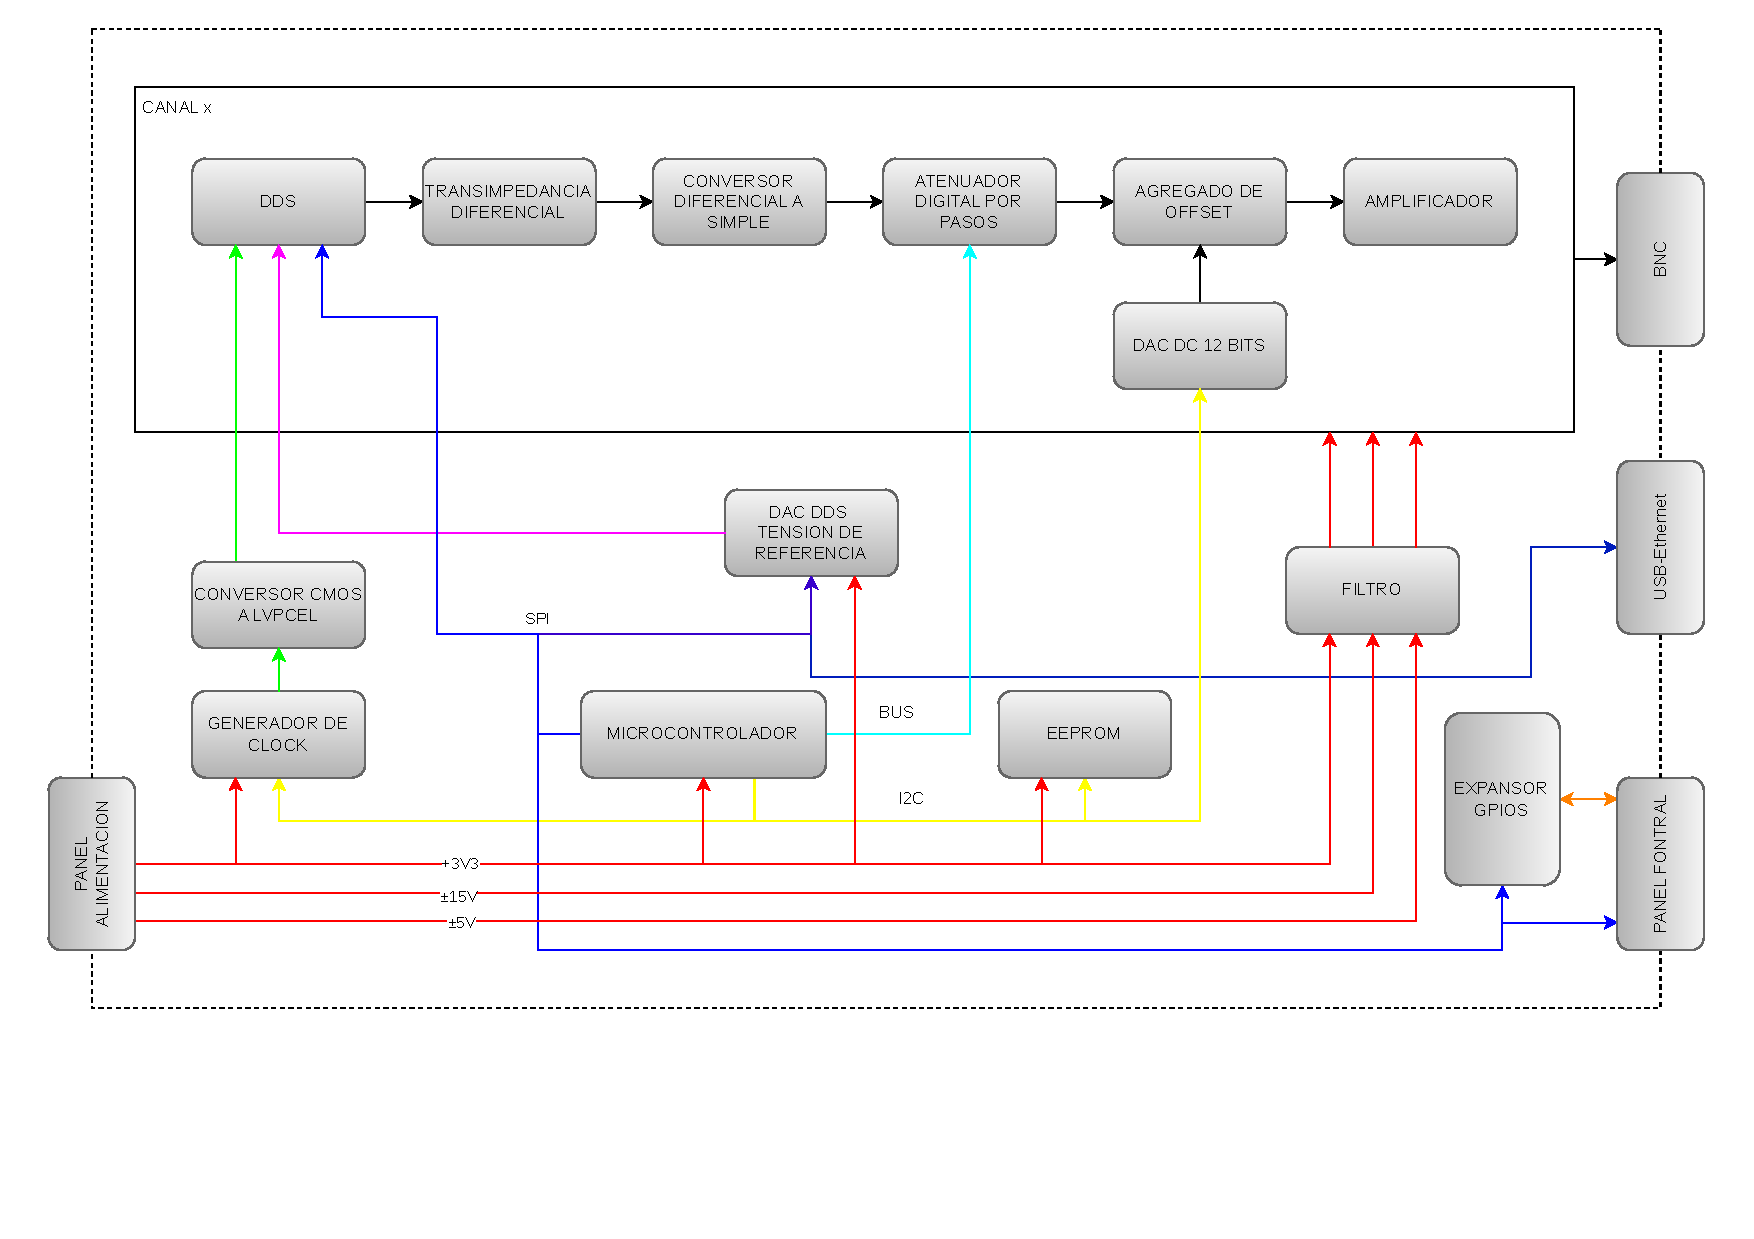
\includegraphics[width=0.8\linewidth]{img/AWG_DDS.pdf}
%	\caption{Diagrama en bloques del Hardware del Generador de Funciones Arbitrarias de la Placa de Control.}
%	\label{fig:awgdds}
%\end{figure}

\begin{sidewaysfigure}
	\centering
	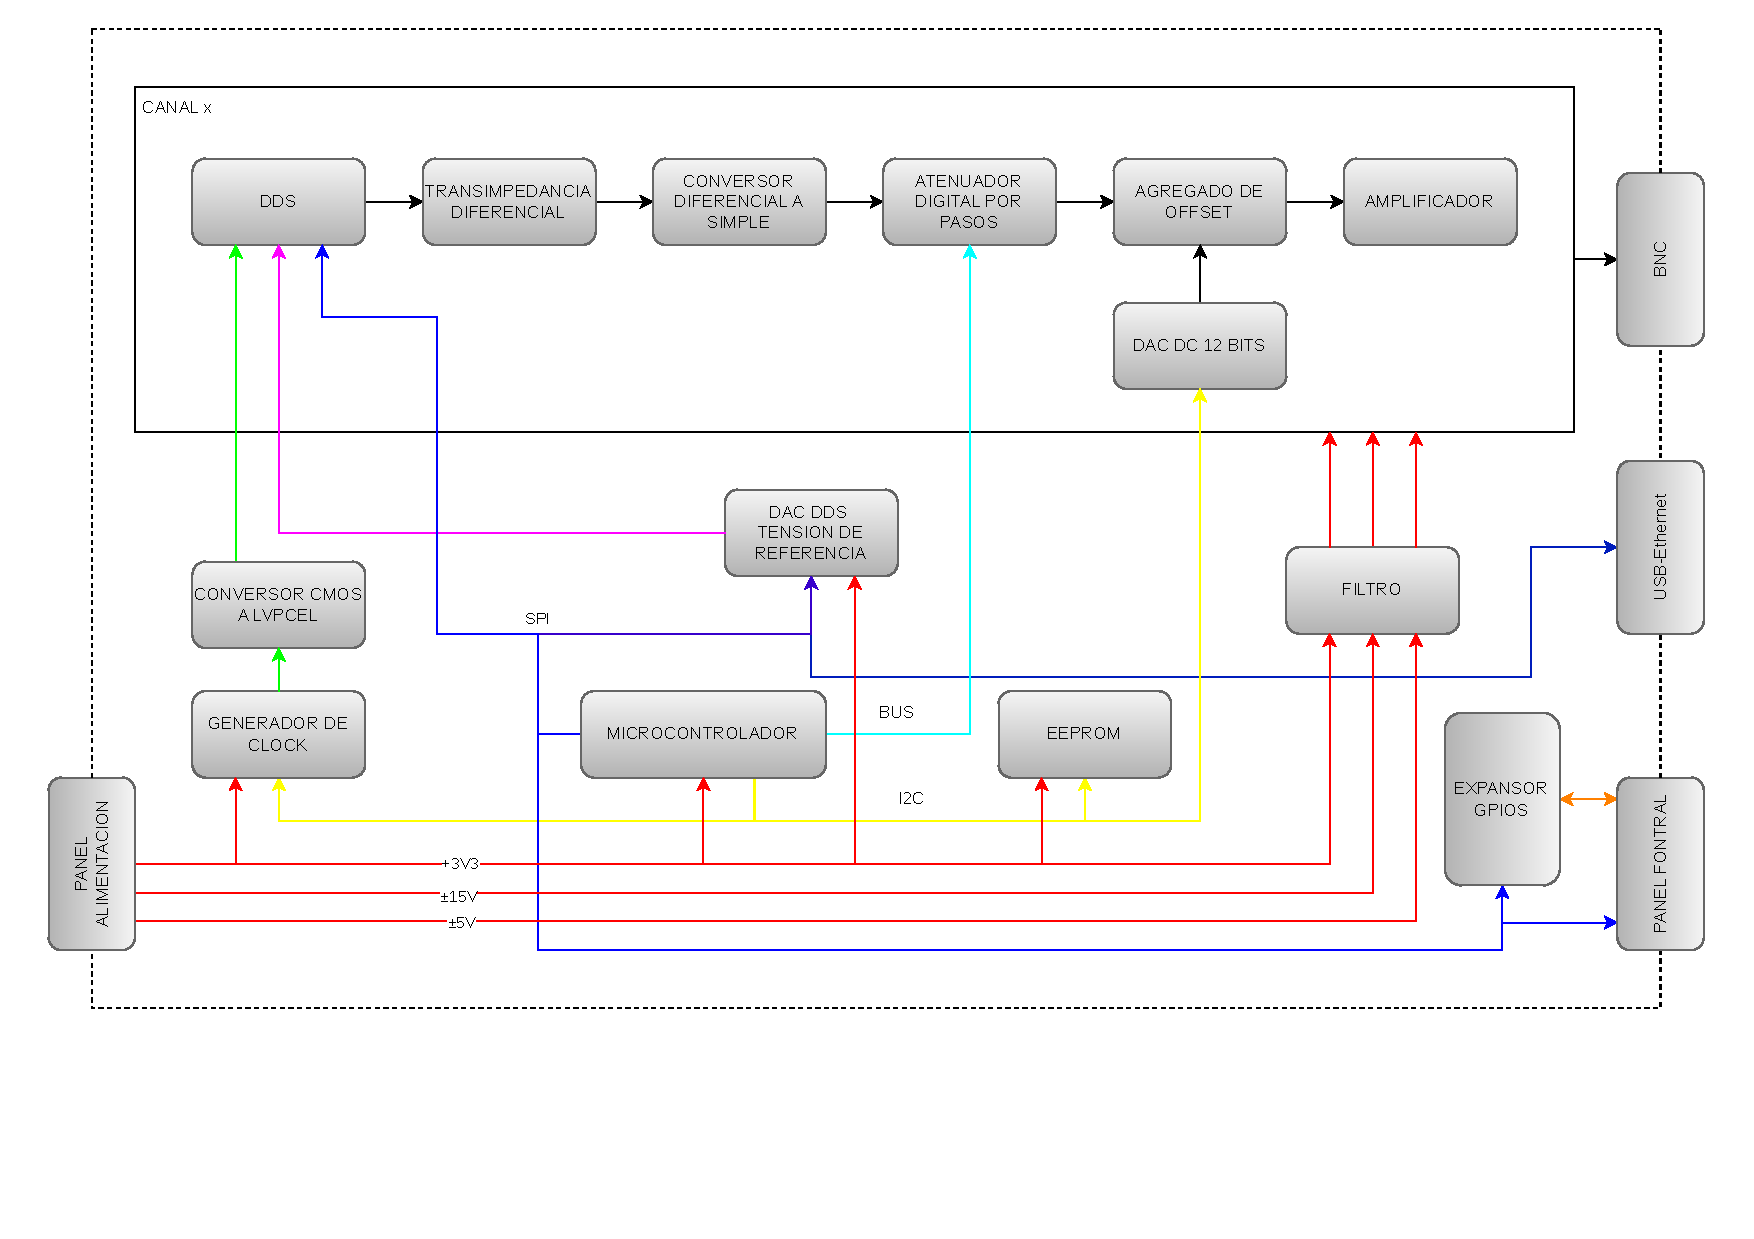
\includegraphics[width=\textheight]{img/AWG_DDS.pdf}
	\caption{Diagrama en bloques del Hardware del Generador de Funciones Arbitrarias de la Placa de Control.}
	\label{fig:awgdds}
\end{sidewaysfigure}


\begin{figure}[H]
	\centering
	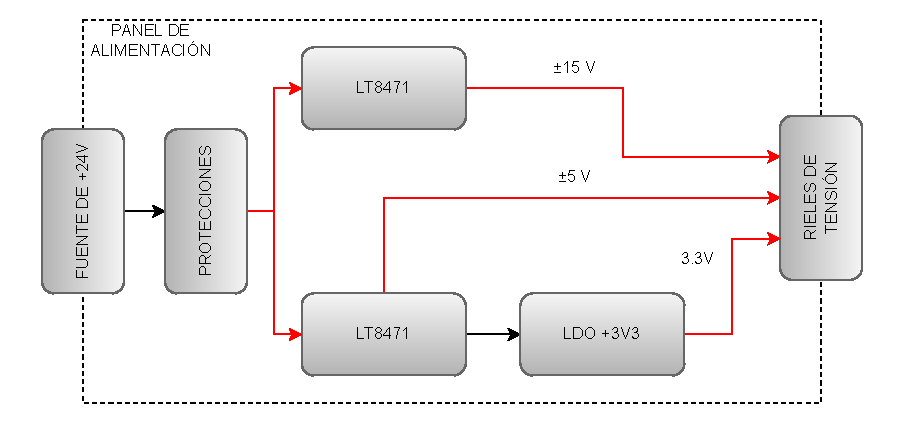
\includegraphics[width=0.7\linewidth]{img/PanelAlimentacionDDS}
	\caption{Diagrama en bloques de la Placa de Alimentación.}
	\label{fig:panelalimentaciondds}
\end{figure}

Se procede a continuación con la explicación detallada de cada diagrama en bloques, comenzando desde la placa de control hasta la placa de alimentación.

\subsection{Diagrama en bloques de la placa de control}

\paragraph{Núcleo de síntesis DDS:} Bloque encargado de generar las muestras digitales correspondientes a la forma de onda seleccionada, permitiendo control de frecuencia, fase y forma arbitraria. En referencia a la Tabla \ref{tab:panorama_dds} se tiene un salida de corriente diferencial para DDS de prestaciones medianas.

Los requisitos mínimos del bloque DDS son:

\begin{itemize}[label=\textbullet]
	\item Resolución del DAC interno $\geq 14$ bits.
	\item Frecuencia máxima de salida senoidal $\geq 20$ MHz.
	\item Frecuencia de clock máxima $\geq 150$ MHz.
	\item Capacidad de generación de formas arbitrarias mediante memoria interna o mecanismo equivalente.
	\item Control programable de frecuencia, fase y amplitud.
	\item Resolución de frecuencia $\leq 1$ Hz.
	\item Interfaz de control digital SPI o equivalente.
	\item Salida diferencial o compatible con una etapa externa de conversión corriente/tensión.
\end{itemize}

\paragraph{Unidad de control digital (Microcontrolador):}
La unidad de control digital constituye el núcleo de procesamiento del sistema, encargándose de la gestión de la lógica principal, configuración del bloque de síntesis, control de periféricos e interfaz con el usuario.

El microcontrolador seleccionado deberá cumplir con los siguientes requisitos mínimos:

\begin{itemize}[label=\textbullet]
	\item Frecuencia de operación $\geq$ 100 MHz.
	\item Memoria RAM interna suficiente para manejo de buffers y estructuras de configuración (mínimo 128 kB recomendados).
	\item Memoria no volátil interna/externa para almacenamiento de firmware.
	\item Interfaz SPI.
	\item Interfaz I\textsuperscript{2}C.
	\item Múltiples temporizadores de propósito general.
	\item Interfaz USB nativa integrada.
	\item Controlador Ethernet externo compatible (mediante SPI o interfaz dedicada).
	\item Cantidad mínima de 30 GPIO configurables.
	\item Soporte para operación en entorno con sistema operativo embebido (RTOS) o scheduler equivalente.
	\item Arquitectura de 32 bits.
\end{itemize}

%Una parte importante de la placa de control, es el microcontrolador que vamos a utilizar, el cual se va a encargar de manejar la lógica central de nuestro instrumento. De esta manera el microcontrolador funciona como el cerebro y el DDS como el corazón de nuestro equipo, enviando el conjunto de comandos necesarios para que se generen las señales que correspondan. En particular utilizamos el \textbf{RP2040} \cite{RaspberryPi_RP2040_Datasheet}, dado que se trata de un integrado que posee una velocidad de trabajo de hasta 130 MHz y una amplia memoria RAM. Elegimos este en comparación con otro, como el ESP32, dado que se poseía de antemano mayor experiencia con este por trabajos previos y además un dispositivo de depuración SWD ya adquirido.
\paragraph{Etapa de transimpedancia diferencial:} Convierte la señal de corriente diferencial proveniente del DDS en una señal de tensión diferencial adecuada para su posterior procesamiento.

Los requisitos mínimos de esta etapa son:

\begin{itemize}[label=\textbullet]
	\item Ancho de banda suficiente para operar hasta 15 MHz sin atenuación significativa.
	\item Slew Rate $\geq 400$ V/$\mu$s.
	\item Bajo ruido agregado.
	\item Buena linealidad en todo el rango dinámico.
	\item Capacidad de operación diferencial.
\end{itemize}

\paragraph{Etapa de conversor de tensión diferencial a simple:} Convierte la tensión diferencial proveniente de la anterior a una tensión de tipo simple, permitiendo adaptarle un conjunto de acondicionamientos de acuerdo a las especificaciones mencionadas.

Los requisitos mínimos de esta etapa son:

\begin{itemize}[label=\textbullet]
	\item Ancho de banda $\geq 100$ MHz.
	\item Slew Rate $\geq 800$ V/$\mu$s.
	\item Baja distorsión armónica en el rango operativo.
	\item Bajo nivel de ruido agregado.
	\item Buena precisión en la conversión diferencial–simple.
\end{itemize}

\paragraph{Control de amplitud (ajuste grueso):}
El sistema deberá incorporar un bloque de atenuación programable que permita ajustar la amplitud de la señal en pasos discretos dentro del rango especificado.

Los requisitos mínimos del bloque de atenuación son:

\begin{itemize}[label=\textbullet]
	\item Rango de atenuación $\geq 30$ dB.
	\item Resolución de paso $\leq 1$ dB.
	\item Operación en el rango de frecuencias del instrumento $\geq$ 50 MHz.
	\item Baja distorsión armónica introducida.
	\item Control digital programable.
\end{itemize}

%\paragraph{Etapa de atenuador digital por pasos:} Permite generar un ajuste grueso de amplitud de la señal previa para su posterior amplificación. Debe adaptarse las impedancias vistas por el integrado para que funcione de manera adecuada.

%Una características importante, es que el usuario pueda variar la amplitud de salida en un rango delimitado por las especificaciones del equipo. Para esto mismo se optó por producir una variación de amplitud con un \textit{ajuste grueso }y un \textit{ajuste fino}. El ajuste grueso se realiza en esta etapa mediante un Atenuador Digital por Pasos (\textbf{DSA}), que es ampliamente utilizado en \textbf{RF}. En los generadores comerciales (antiguos o económicos) es común tener un conjunto de relés que van conmutando de manera de generar una atenuación determinada con rangos de resistencias. Si bien puede implementarse esa solución, el problema es que ocupa mucho espacio y depende en gran medida de la resistencias elegidas, dada por su distorsión, tolerancia, etc. Por esto mismo la propuesta de utilizar un \textbf{DSA}, aunque es mas costosa, es una solución mas acorde y precisa. En particular luego de un proceso de investigación se va a hacer uso del DSA \textbf{PE4312} \cite{pSemi_PE4312_Datasheet} que provee varios rangos de atenuación que van desde los 0.5 db hasta los 30.5 db y trabaja hasta una frecuencia de 4 GHz, con lo que queda cubierto para todo el rango de frecuencias especificadas.

\paragraph{Etapa de Offset:} Agrega un nivel de DC a la señal de salida del atenuador digital por pasos, según la configuración del usuario.

Los requisitos mínimos del bloque de offset son:

\begin{itemize}[label=\textbullet]
	\item Rango de offset ajustable compatible con $\pm 5$ V en la salida.
	\item Resolución mínima de ajuste $\leq 100$ mV.
	\item Bajo nivel de ruido agregado.
	\item Buena estabilidad térmica.
	\item Linealidad adecuada en todo el rango operativo.
	\item Control digital programable mediante SPI o I\textsuperscript{2}C.
	\item Capacidad de operación bipolar.
\end{itemize}

%Una vez que se tiene la forma de onda acoplada en AC y con un valor de atenuación correspondiente, es necesario aplicarle, si corresponde, el valor de DC que el usuario configure. Para esto mismo se hace uso de un conversor de digital a analógico de la marca Texas Instruments \textbf{MCP4725} \cite{Microchip_MCP4725_Datasheet}. Este \textbf{DAC }posee una sola salida con \textbf{resolución de 12 bits }y es manipulado por \textbf{I2C}. Dado que se tienen dos canales es necesario utilizar dos integrados de estos, uno para canal. Además una especificación importante es que el usuario tiene la posibilidad de ingresar un valor de continua tanto positivo como negativo, sin embargo el valor de tensión que produce a la salida del DAC mencionado únicamente es positivo. Entonces es necesario un circuito de adaptación que permita convertir este valor positivo, en un valor de tipo bipolar. Cabe aclarar que existen comercialmente DACs que permiten obtener a su salida un valor de tensión bipolar, pero el costo de estos es tan alto que supera con creces el obtenido al comprar los componentes necesarios para el circuito convertidor antes mencionado mas el \textbf{MCP4725}.

\paragraph{Etapa de amplificación de salida:}
La etapa de salida es responsable de proporcionar el nivel final de tensión y corriente especificado, así como la adaptación a impedancia estándar de 50 $\Omega$.

El amplificador o conjunto de amplificadores seleccionados deberán cumplir con los siguientes requisitos mínimos:

\begin{itemize}[label=\textbullet]
	\item Capacidad de excursión de salida compatible con 20 Vpp en alta impedancia.
	\item Corriente de salida $\geq 100$ mA.
	\item Ancho de banda en lazo cerrado $\geq 50$ MHz.
	\item Slew Rate suficiente para señales de hasta 10 MHz (SR $\geq 4000$ V/$\mu$s recomendado).
	\item Operación con rieles de alimentación simétricos.
	\item Estabilidad con carga de 50 $\Omega$.
\end{itemize}

%\paragraph{Amplificador:} Amplifica la señal mixta proveniente de la etapa de offset, generando una amplitud máxima de 20 Vpp y 5 Vp de offset. También adapta la impedancia de salida a 50 $\Omega$.

%Esta última etapa consiste en una amplificación final de la señal previa, con una ganancia que permita obtener a su salida una amplitud máxima de 20 Vpp y 5 Vp de offset. Además, como se mencionó en las especificaciones del comienzo la impedancia de salida, $Z_o = 50 \ \Omega$ y la corriente de salida máxima, $I_{omax} = \pm 620$ mA. Para esto mismo se hace uso de dos amplificadores operacionales \textbf{THS3091} \cite{TI_THS3091_Datasheet}. Cada uno puede proveer una corriente máxima de $\pm$310 mA y a la salida de cada AO se le añade una resistencia en serie de 100 $\Omega$ al 0.1\%. Luego cada salida es unida para lograr lo antes mencionado.

\paragraph{Generación de reloj:}
El núcleo de síntesis digital requiere una señal de reloj estable y de baja fluctuación temporal (jitter), que determine la frecuencia de muestreo del sistema.

El generador de clock deberá cumplir con los siguientes requisitos:

\begin{itemize}[label=\textbullet]
	\item Frecuencia de salida $\geq 150$ MHz.
	\item Estabilidad adecuada para aplicaciones de instrumentación.
	\item Bajo jitter para preservar la calidad espectral de la señal generada.
	\item Posibilidad de configuración o ajuste programable.
\end{itemize}

%\paragraph{Generador de reloj y acondicionamiento de señal:}
%El núcleo de síntesis digital requiere una señal de reloj de alta estabilidad para su correcto funcionamiento. Este bloque tiene como función generar y distribuir la señal de clock necesaria para la sincronización interna del sistema, permitiendo ajustar la frecuencia de operación dentro del rango especificado. Asimismo, se contempla el acondicionamiento eléctrico de dicha señal para garantizar compatibilidad con los niveles lógicos requeridos por el bloque de síntesis.

\paragraph{Memoria no volátil:}
Con el objetivo de brindar al usuario la posibilidad de almacenar configuraciones, parámetros operativos y tablas de muestras correspondientes a formas de onda arbitrarias, el sistema incorpora un bloque de memoria no volátil. Este módulo permite conservar información incluso ante la pérdida de alimentación, facilitando la recuperación de estados previos y configuraciones personalizadas.

\paragraph{Interfaz de expansión de entradas/salidas:}
La interfaz hombre–máquina (HMI) requiere la gestión de múltiples señales provenientes del panel frontal, tales como pulsadores, encoder rotativo y display. Para ello se incorpora un bloque de expansión de entradas/salidas digitales, cuya función es ampliar la cantidad de líneas disponibles y permitir la correcta lectura y control de los periféricos asociados a la interacción con el usuario.

\paragraph{Interfaz USB:}
Permite la comunicación directa con una computadora u otros dispositivos externos para configuración remota, actualización de firmware y posible transferencia de datos. Este bloque amplía las capacidades del instrumento en entornos de laboratorio y automatización.

\paragraph{Interfaz Ethernet:}
El sistema incorpora una interfaz de comunicación Ethernet.

Los requisitos mínimos del bloque Ethernet son:

\begin{itemize}[label=\textbullet]
	\item Compatibilidad con estándar 10/100 Mbps.
	\item Soporte para pila TCP/IP.
	\item Interfaz de conexión con la unidad de control mediante bus digital dedicado (SPI o equivalente).
	\item Aislamiento y protección adecuados para operación en red.
\end{itemize}

\paragraph{Filtrado y desacople:}
Dado que el sistema integra etapas digitales y analógicas en un mismo dispositivo, se implementan estrategias de filtrado y desacople destinadas a minimizar el acoplamiento de ruido entre dominios. Este bloque contempla el aislamiento funcional entre la alimentación digital y analógica, así como la mitigación de interferencias generadas por conmutaciones de alta frecuencia.

%\paragraph{Generador de clock y conversor a LVPCEL:} Como se mencionó en la primera etapa del DDS, es necesario utilizar un reloj para sincronización interna del propio integrado. Por esto mismo se hace uso de un generador de reloj con el circuito integrado conocido \textbf{SI5351} \cite{Skyworks_Si5351_Datasheet}. Este permite producir frecuencias cuadradas desde 2 KHz hasta 260 MHz, utilizando únicamente un oscilador de 25 MHz a 27 MHz y comunicación I2C.
%
%\paragraph{EEPROM:} La idea principal detrás de esta etapa de hardware es poder darle la opción al usuario de guardar un conjunto de parámetros tales como configuraciones preliminares, últimos valores configurados, tablas de muestras (para generar formas de onda arbitrarias), etc. En este caso particular se hace uso de la memoria \textbf{24LC1025T} \cite{Microchip_24LC1025_Datasheet}, dado que posee un espacio de 128 KB, lo que nos permitirá guardar una gran cantidad de formas de onda arbitrarias, así como también configuraciones extras.
%
%\paragraph{Expansor GPIOs:} En el \textbf{panel frontal} se encuentran el conjunto de botoneras, encoder, display y demás periféricos que interactúan con el usuario, siendo este parte del hardware necesario para una interfaz hombre máquina (\textbf{HMI}). La función principal del expansor de gpios es poder manipular un conjunto de 16 pulsadores que realizan diferentes funciones. En este sentido el panel frontal tiene la forma del generador de funciones basado en DDS FY6900 presentado anteriormente. En este caso se hace uso del integrado conocido \textbf{MCP23S17} \cite{Microchip_MCP23S17_Datasheet}, el cual es muy utilizado como expansor de puertos en dispositivos PLC, lo que lo convierte en una de las razones principales por la cual fue elegido.
%
%\paragraph{Filtros:} Dado que se tiene un circuito del tipo \textit{señales mixtas} (porque poseemos señales digitales y analógicas), debemos de alguna manera filtrar las oscilaciones producidas debido a las conmutaciones generadas por componentes de la etapa digital (comunicaciones spi, i2c, uart, entre otras), con respecto a la etapa analógica. En efecto la función principal de este bloque consiste en aislar la alimentación de la etapa digital y la analógica.

\subsection{Diagrama en bloques de la placa de alimentación}

\paragraph{Fuente primaria:}
El sistema es alimentado mediante una fuente de entrada externa de corriente continua. Este bloque proporciona el nivel de tensión principal a partir del cual se generan los rieles secundarios necesarios para el funcionamiento del equipo.

Los requisitos mínimos de la fuente de alimentación son:

\begin{itemize}[label=\textbullet]
	\item Fuente de alimentación de +24 V.
	\item Potencia máxima de entrada de 70 W para alimentar el resto de placas.
	\item Fuente de tipo conmutada con bajo nivel de ripple a la salida.
	\item Buena regulación frente a variaciones de carga.
\end{itemize}

\paragraph{Generación de rieles analógicos:}
Con el fin de alcanzar la amplitud máxima especificada en la salida del instrumento, es necesario disponer de rieles de alimentación simétricos para las etapas analógicas de acondicionamiento y amplificación. Este bloque genera tensiones positivas y negativas adecuadas para permitir excursiones de señal dentro del rango definido en las especificaciones del equipo.

Los requisitos mínimos de estos rieles son:

\begin{itemize}[label=\textbullet]
	\item Generación de tensiones $\pm 15$ V para la etapa de salida.
	\item Generación de tensiones auxiliares $\pm 5$ V para etapas intermedias.
	\item Capacidad de corriente suficiente para operación a carga máxima.
	\item Bajo rizado residual.
	\item Buena regulación frente a variaciones de carga.
\end{itemize}

\paragraph{Generación de riel digital:}
Las etapas digitales del sistema, tales como la unidad de control, memoria e interfaces de comunicación, requieren una tensión regulada de menor nivel. Para ello se incorpora un bloque de regulación dedicado que garantiza estabilidad y bajo nivel de ruido en el dominio digital.

\begin{itemize}[label=\textbullet]
	\item Generación de riel de 3.3 V.
	\item Bajo nivel de ruido.
	\item Estabilidad adecuada para sistemas digitales de alta velocidad.
\end{itemize}

\paragraph{Separación de dominios y filtrado:}
Dado que el instrumento integra etapas analógicas de alta velocidad junto con circuitos digitales de conmutación, se implementa una separación funcional entre dominios de alimentación. Esta arquitectura contempla técnicas de filtrado, desacople y distribución adecuada de masa para minimizar el acoplamiento de ruido y preservar la integridad de la señal.

%\paragraph{Fuente de alimentación de 24V:} La placa de alimentación es alimentada con una fuente de tipo conmutada de 24V. Se utilizó este tipo de fuente en particular, dado que es de bajo coste y con alta eficiencia en comparación con un fuente lineal.
%
%\paragraph{LT8471:} Estos módulos son los encargados de producir los rieles de tensión necesarios para utilizar en la placa de control y poder generar la amplitud de salida configurada por el usuario. Como se menciona en la especificaciones el máximo valor de amplitud de pico es de 15 V para un carga de alta impedancia (High-Z). Con lo cual debemos generar rieles de alimentación de $\pm$15 V y $\pm$5 V para pre-amplificación. Además es necesario alimentar circuitos integrados digitales, tales como microcontrolador, memoria eeprom, dacs, etc. Con lo cual es necesario un riel extra de 3.3 V. Cada integrado \textbf{LT8471} \cite{ADI_LT8471_Datasheet} es capaz de generar dos rieles simétricos, por lo que es necesario dos integrados para poder generar los niveles adecuados.
%
%\paragraph{LDO 3.3V:} Por último se tiene un regulador de baja caída de tensión (\textbf{LDO}), el cual es capaz de generar un nivel de tensión adecuado para los integrados de la etapa digital.

\subsection{Firmware}

La arquitectura de firmware se diseña con el objetivo de garantizar modularidad, escalabilidad y mantenimiento simplificado del sistema. Para ello se adopta una estructura organizada en bloques funcionales claramente definidos, como se muestra en la Figura \ref{fig:firmwaredb}.

\subsubsection{Arquitectura de software}

El firmware se estructura bajo un modelo modular, donde cada bloque representa una función específica del sistema. Esta organización permite desacoplar la lógica de alto nivel del control directo del hardware, favoreciendo la reutilización de código y la claridad estructural.

La arquitectura contempla la ejecución concurrente de tareas relacionadas con la interfaz de usuario, actualización de parámetros y control de periféricos, permitiendo una respuesta fluida ante la interacción del usuario.

\subsubsection{Descripción de bloques}

\paragraph{Lógica principal:}
Representa el nivel jerárquico superior del sistema. Gestiona la configuración global del instrumento, coordina la interacción entre módulos y mantiene el estado general del equipo.

\paragraph{Control de periféricos:}
Actúa como interfaz entre los elementos físicos de interacción (pulsadores, encoder, display) y la lógica principal. Su función es interpretar eventos externos y convertirlos en acciones internas del sistema.

\paragraph{Selección de configuración:}
Procesa las órdenes provenientes de la lógica principal y determina qué parámetro del instrumento debe modificarse (frecuencia, amplitud, fase, tipo de señal, entre otros).

\paragraph{Configuración de hardware:}
Recibe los valores finales a aplicar y se encarga de actualizar los bloques físicos correspondientes del sistema, garantizando que los cambios solicitados por el usuario se reflejen en la señal de salida.
%
%\subsection{Firmware}
%Para concluir con la forma de implementación se hace referencia a la estructura de programación que debe seguirse con el objetivo de mantener un código que sea legible y escalable. Por esto mismo se procedió a realizar un diagrama en bloques que se muestra a continuación. Posteriormente describiremos a grandes rasgos que hace cada etapa.

\begin{sidewaysfigure}
	\centering
	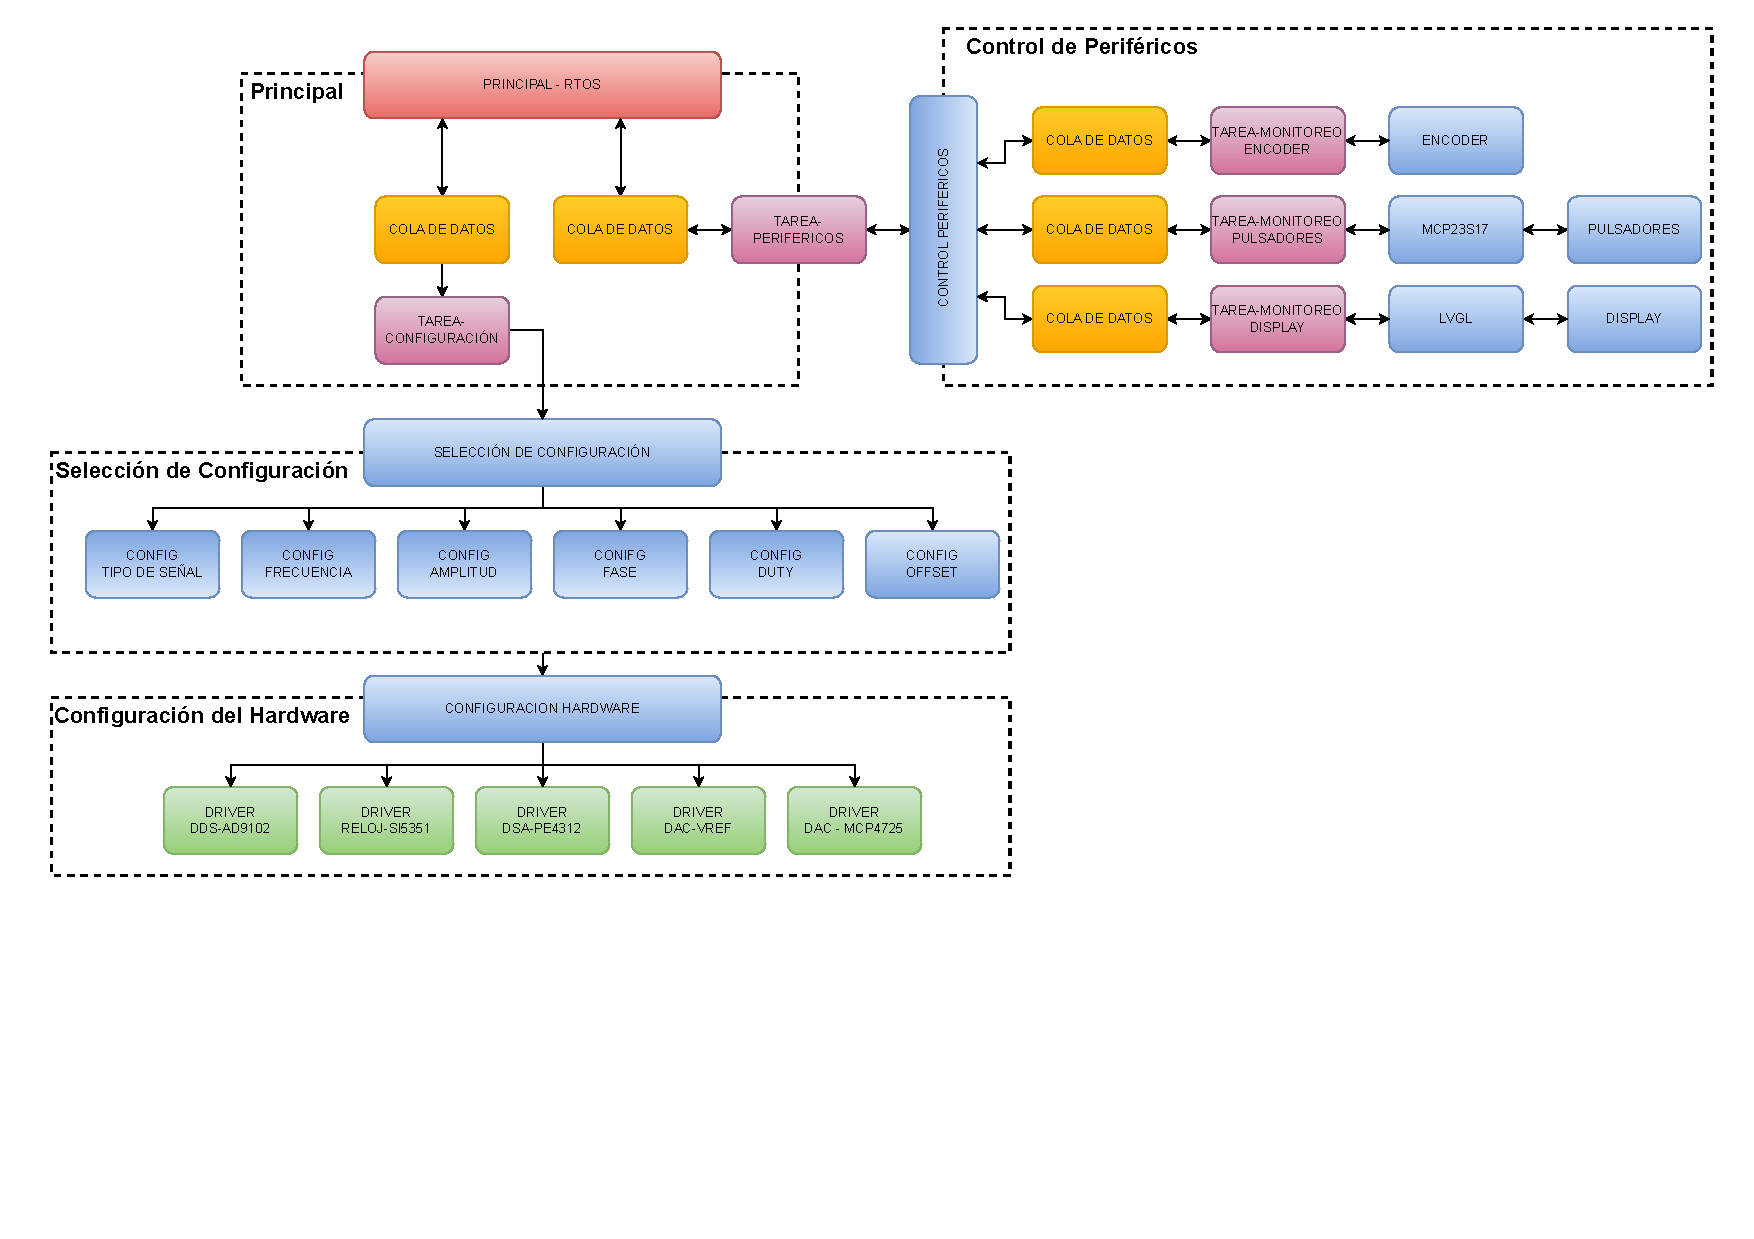
\includegraphics[
	width=\textheight, % usa el "alto" de la página porque está rotada
	clip,
	trim={0cm 5cm 0cm 0cm}
	]{img/Firmware_DB.drawio}
	\caption{Diagrama en bloques del firmware.}
	\label{fig:firmwaredb}
\end{sidewaysfigure}

%\subsubsection{Programación orientada a Objetos}
%La Programación Orientada a Objetos (\textbf{POO}) es un paradigma de programación basado en organizar el software/firmware alrededor de ``objetos'' (datos) y sus comportamientos (métodos), en lugar de funciones lógicas. Reduce errores, promueve la reutilización de código y facilita el mantenimiento de sistemas complejos mediante conceptos como \textit{clases, herencia, encapsulamiento} y \textit{polimorfismo}. 
%
%En el caso de nuestro proyecto la programación orientada a objetos nos va a ser de gran utilidad, porque nos permite poder tener una representación de un ``objeto'' que va a representar algo físico en nuestro circuito. Dicho de otra manera cada objeto va a ser una porción del hardware. Por ejemplo podríamos tener un objeto del tipo \textbf{amplitud}, que cuando el usuario varíe un conjunto de parámetros, esto se vea reflejado en enviar un conjunto de señales al atenuador digital por pasos (DSA), para que la amplitud máxima de la señal de salida varíe. Entonces teniendo este concepto en mente procedemos a la explicación del diagrama en bloques del firmware, Figura \ref{fig:firmwaredb}.

%\subsubsection{Diagrama en bloques del Firmware}
%En este sección se explicarán los elementos más importantes del diagrama en bloques, que pueden visualizarse en la Figura \ref{fig:firmwaredb}.
%
%\paragraph{Principal-RTOS:} Este bloque representa la jerarquía mas alta del código. Se encuentran las configuraciones, declaraciones de objetos y lógica principal. Como se menciona en el nombre puede verse que se va a utilizar un RTOS (a definir), una justificación clara de esto, es que nos permite poder hacer uso de tareas que se ejecuten en forma \textbf{concurrente}. Un ejemplo de estas tareas son la mostradas en color rosa \textbf{TAREA ENCODER}, \textbf{TAREA MONITOREO PULSADORES}, \textbf{TAREA DISPLAY}. Esto nos permite en cierta manera manejar diferentes periféricos de forma paralela, evaluar si hubo cambios o generarlos, si fuese necesario, sin la necesidad de hacer grandes fragmentos de código, dado que son elementos físicos completamente diferentes.
%
%\paragraph{Control de Periféricos:} Su función es actuar como un intermediario entre el mundo externo, en el que se encuentra el usuario y modifica periféricos, y la lógica principal que sería el bloque explicado anteriormente.
%
%\paragraph{Selección de Configuración:} Esta bloque se encarga de procesar la información que ingresa desde la lógica principal, presentada al comienzo, para conmutar entre el tipo de configuración que quiere realizar el usuario. Al final de las explicaciones de lo bloques se presentan un ejemplo globalizar que muestra como cada uno interactúa con el resto, formando un sistema completo.
%
%\paragraph{Configuración del Hardware:} Esta se encarga de recibir un conjunto de valores a modificar y conocimiento de antemano que tipo de configuración es la que está seleccionada, se procede a interactuar con el driver que corresponda, para posteriormente generar el conjunto de señales adecuadas para el circuito integrado correspondiente.
%
%Para tener una visión mas clara de como interactúan todos estos bloques principales se menciona un ejemplo. Supongamos que el usuario quiere modificar la amplitud de salida en el canal 1. Para esto, lo primero que debe hacer es seleccionar dicho canal, pulsando sobre el botón correspondiente. Esta información pasa por el bloque de \textit{Control de Periféricos} que la procesa, agrega algún tipo de parámetro y luego la manda hacia el bloque \textit{Principal}. Este mismo modifica su lógica, informando al siguiente bloque \textit{Selección de Configuración}, cual tipo es seleccionada. Posteriormente el usuario interacciona con el \textit{encoder}, esto se envía por los mismos bloques, ya mencionados, hasta llegar al actual, el cual informa al bloque \textit{Configuración del Hardware} que debe existir un cambio a nivel físico y por lo tanto este mismo actúa en consecuencia sobre el driver correspondiente.

